\section{Results}
\label{sec:results}

\paragraph{Main Results.} The performance on our generated tasks is consistently and substantially lower against \taubench (Verified version, \tbv), with relative drops ($\Delta\%$) ranging from $-5\%$ to $-80\%$, depending on the agent and domain (Table~\ref{tab:main-results}). We compared the performance of $11$ agent--user pairs across three domains. The degradation is particularly striking for LLMs that appear to have nearly saturated \tbv: Gemini-$3$-flash, for instance, achieves $0.82$--$0.94$ on \tbv across Airline, Retail, and Telecom domains (except Airline with Gemini-$3$-Flash user), yet drops to $0.28$--$0.61$ on \ourbenchmark. This suggests that the high \tbv scores may reflect benchmark saturation rather than robust task-solving ability. \ourbenchmark exposes gaps that the original benchmark no longer captures, enabling differentiation among state-of-the-art LLMs and supporting continuous, scalable evaluation.

\begin{figure*}[t]
    \centering
    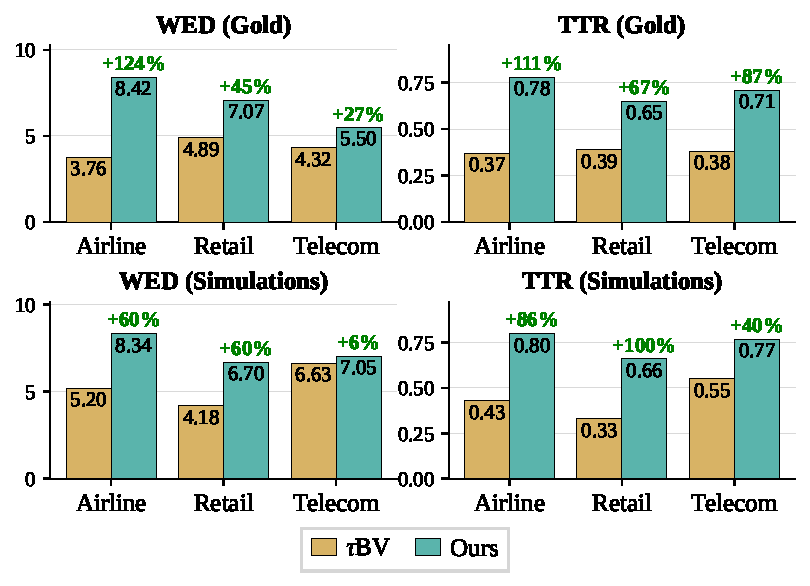
\includegraphics[width=0.55\textwidth]{assets/figures/metric_grid.pdf}
    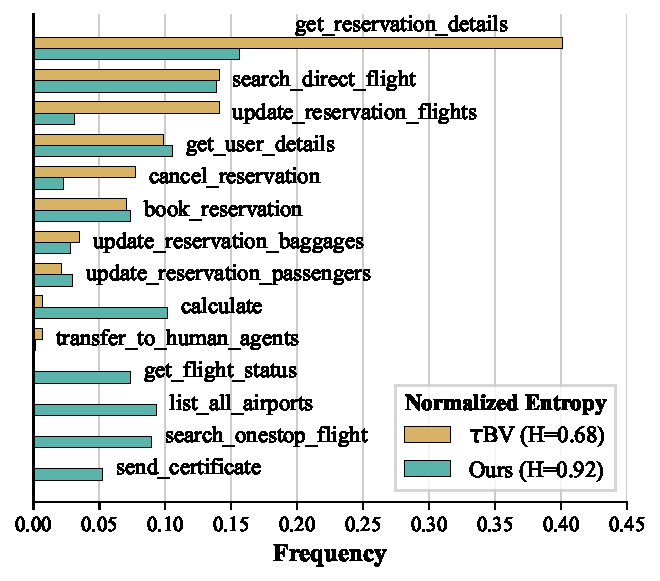
\includegraphics[width=0.44\textwidth]{assets/figures/tool_frequency.pdf}
\caption{\textbf{Coverage Metrics (Left):} Weighted Edit Distance (WED) and Type-Token Ratio (TTR, averaged over $n \in \{2,\dots,6\}$), computed for both gold sequences (top) and sequences extracted from successful simulation trajectories (bottom). \textbf{Airline Tool Frequency (Right):} Distribution of tools in gold sequences. The $\tau\text{BV}$ distribution is notably more skewed. Other domains in Figure~\ref{fig:diversity-combined}.}
    \label{fig:coverage_fig}
\vspace{-1.25em}
\end{figure*}

\paragraph{Harder Tasks with Broader Coverage.}
We compare the coverage and diversity of \ourbenchmark against \tbv, adopting $n$-gram diversity metrics from the NLP literature.
In Figure~\ref{fig:coverage_fig} (left), we present two metrics.
The first is the weighted edit distance (WED) between the tool sequences, capturing the structural dissimilarity of the required execution paths. The second is the Type-Token Ratio (TTR), the fraction of unique $n$-grams ($n\in\{2,...,6\}$) among all $n$-gram occurrences, capturing how much of the available tool-combination space is exercised. We also compute these metrics on tool sequences extracted from successful simulations (see Appendix~\ref{app:sequence-metrics-full}).
Our tasks show consistent and substantial gains across all three domains: WED increases by up to $124\%$, TTR by up to $111\%$, 
and the tool-frequency distribution is markedly less skewed with entropy increased by $35\%$ (Figure~\ref{fig:coverage_fig}, right).
These results indicate our tasks require agents to follow more varied and distinct execution paths. A more detailed analysis (Appendix~\ref{app:sequence-metrics-full}) applies additional metrics; across all domains, metrics, and sequence sources, our tasks are consistently more challenging and diverse.

\subsection{Method Analysis}
\label{sub:method_analysis}

In this subsection, we analyze key design choices of TASTE and provide empirical justifications. 

\paragraph{Ablation of the Adaptive Contrastive $n$-gram Model.} 
The goal of using $n$-gram model in TASTE is to sample from the space of valid tool sequences while maintaining broad coverage. We achieved $86.7\%$ validity rate with our full trained model compared to uniform tool sampling ($6.7\%$), illustrates the overall impact of our design.
We extend the standard model in two ways: through adaptive online training and the integration of contrastive negative evidence. Figure~\ref{fig:method_analysis} (left) presents an ablation study of the model's components within the airline domain. Adaptive online training is essential: even when the model is initialized with $n$-grams from \tbv tasks, the validity rate without training reaches only $16.7\%$, whereas iterative training steadily improves it (as shown by the dark red line). The contrastive formulation provides a complementary and substantial gain. Training with negative evidence (i.e., ingesting invalid $n$-grams into $C^-$ to avoid sampling them) improves the validity rate by $10$ points at $k\!=\!400$, and by $20$ points at $k=800$. Finally, evaluating the final model ($k\!=\!3000$) trained with negative evidence to examine the impact of $\lambda_{\text{neg}}$ on sampling reveals an additional $10$-point improvement. In total, our design choices raise the validity rate from $6.7\%$ to $86.7\%$. This ${\sim}\!13{\times}$ improvement enables us to sample a large pool of plausibly valid candidates.

\paragraph{Evaluation of the Verifier Agent.} To validate generated tasks, we apply a hint-assisted verifier agent, which attempts to complete each task given a shuffled, partially masked list of gold tool calls. A task is deemed valid if the agent succeeds. To evaluate its reliability, we construct a validation dataset by comparing each original task from \taubench with its corresponding entry in \taubenchverified, and assign these labels: \emph{valid:} if the task was not modified in Verified; \emph{invalid:} if the fix involved changing an action or substantially rewriting the instruction; tasks with minor fixes (e.g., capitalizing a single word) are excluded. This yields $50$ Airline tasks ($8$ invalid) and $86$ Retail tasks ($9$ invalid). The verifier agent achieves precision of $1.0$ and $0.97$ and recall of $0.75$ and $0.83$ in Airline and Retail, respectively. Accordingly, the agent may reject some valid tasks (recall $<0.9$), but the near-perfect precision ensures any task passing is almost certainly valid. Finally, we also manually examined all tasks from \ourbenchmark on which none of the evaluated agent-user pairs succeeded ($1$ Airline, $7$ Retail, and $7$ Telecom). All $15$ tasks were found to be valid; failures were due to agent mistakes.

\paragraph{Creating Difficult Tasks.} TASTE increases task difficulty through task evolution. In Figure~\ref{fig:method_analysis} (right), we compare base tasks in the Airline and Retail domains with evolved versions, using two agents and the Gemini-$3$-Flash user simulator. As shown, success rates are $36$--$55$\% lower when tasks are evolved by Gemini-$3$, and $16$--$37$\% lower when evolved by GPT-$5.2$, leading us to select Gemini-$3$. Difficulty can also be controlled through tool-sequence length and the read-to-write tool ratio during TASTE's sampling and selection stages. In Figure~\ref{fig:difficulty-desiderata} (Appendix~\ref{app:difficulty-desiderata}), we compare two tiers of tasks (top $50\%$ vs. bottom $50\%$ by length and tool type ratio). As shown, performance on longer tasks is $30\%$ lower on average (across all agent-user pairs and domains) and $43\%$ lower on write-heavy tasks. This suggests that TASTE can be used to generate even harder tasks in the future, should existing benchmarks saturate.

\begin{figure*}[t]
    \centering
    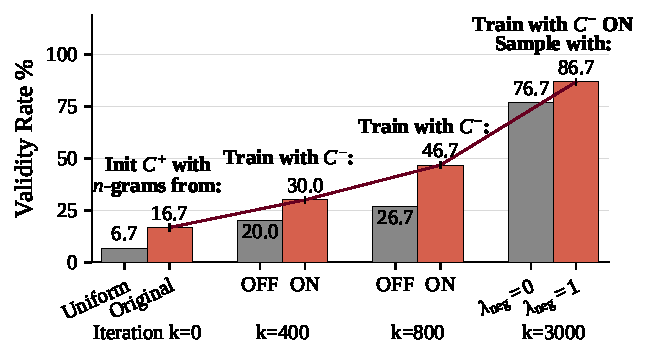
\includegraphics[width=0.48\textwidth]{assets/figures/validity_rate.pdf}
    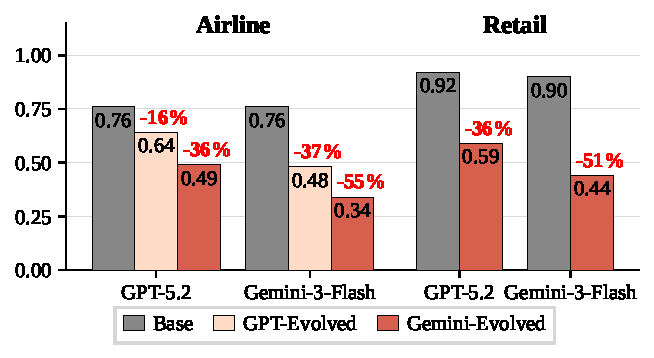
\includegraphics[width=0.48\textwidth]{assets/figures/eval_barplot.pdf}
    \caption{\textbf{$n$-gram Model (Left):} Acceptance rate of sampled sequences across training stages and model configurations on the Airline domain. The dark red line traces the full adaptive contrastive model across iterations. \textbf{Task Evolution (Right):} Success rate of two agents (Gemini-3-Flash as the user simulator) on base vs.\ evolved tasks. Tasks are evolved by either GPT-5.2 or Gemini-3.}
    \label{fig:method_analysis}
\vspace{-1em}
\end{figure*}

